\chapter{Introduction}
\label{ch:intro}

The nature of dark matter (DM) remains one of the major unsolved problems in physics. Originally inferred through its gravitational influence on galaxies and clusters, a rich body of evidence has accumulated over the last four decades firmly establishing its existence. All of the evidence, however, comes from inferring dark matter's presence uniquely through its gravitational effects. Much else about it remains an open question: Does dark matter consist  of a fundamental particle? What is its mass? Could there be an entire dark sector, akin to our own Standard Model? How does dark matter interact with the Standard Model? Answering these questions represents a giant ongoing effort that draws from a rich body of theoretical and experimental work, as well as major input from the computational and numerical side. Fortunately, we are at the dawn of a data-driven era in astrophysics and cosmology with great potential to elucidate the nature of dark matter. A large number of ongoing and forthcoming experiments, both in the lab and in the sky, as well as increasingly open approach to data availability present great promise in this direction. 

Dark matter plays a central role in many subfields of particle physics, astrophysics and cosmology. Understanding its nature and interactions would have far reaching consequences, as there is no concrete explanation within the frameworks of the Standard Models of particle physics and cosmology. It would represent a paradigm shift in those fields and provide major insights into fundamental physics beyond the Standard Model, as well as elucidate the evolution of our Universe and the formation of structures within it. 

% While there exists a proliferation of ideas regarding the particle nature of dark matter, the dominant paradigm over the last three decades has been that of the Weakly Interacting Massive Particle (WIMP), which posits dark matter to consist of a particle with weak-scale interactions with the Standard Model, produced through thermal freeze-out in the early universe. This framework dovetails well, for example, with supersymmetric extensions to the Standard Model where candidates for dark matter can emerge naturally. After briefly describing alternative explanations, in this thesis I will focus exclusively on WIMP searches. I will also focus exclusively on astrophysical searches for WIMPs.

This chapter is organized as follows. In Sec.~\ref{sec:evidence} I will summarize the large body of evidence that points to the existence of dark matter. In Sec.~\ref{sec:particledm} I will describe possible explanations underlying the particle nature of dark matter, describing WIMPs and summarizing alternative explanations. Section~\ref{sec:astrodm} will focus on the astrophysical effort to detect and characterize the nature of DM, in particular using gamma-ray data, and I will describe the theoretical and experimental tools available to us and the status of the field in this context. Finally, in Sec.~\ref{sec:summary} I will describe the organization of the rest of this thesis. % Wherever possible, I will touch upon the historical developments that have paved the way for our current state of understanding of dark matter and our efforts to look for it.

\section{Evidence for Dark Matter}
\label{sec:evidence}

Although dark matter had its inception and development in the 20th century, several scientific problems that philosophically encapsulate the dark matter problem as we see it today had their roots in earlier times. For example, the Aristotelian geometric view of an immutable Universe with the Earth as its center on the other hand offered a clean framework that did not call for additional invisible matter or celestial objects, and was the orthodox viewpoint until Renaissance astronomers conclusively refuted it with observations. Galileo, in the face of significant resistance from the Catholic Church, arguably played the largest role in this and discovered much that was previous unknowable -- including understanding the make-up of the Milky Way as consisting of individual stars rather than nebulous clouds, and observing Saturn's rings and Jupiter's four largest moons. These observations are very much in the spirit of modern dark matter searches -- demonstrating that the Universe can contain invisible forms of matter, and that scientific inquiry and technological developments can play a big role in revealing it to us.

% \subsection{Dynamical Evidence}

Evidence for some yet-unknown form of matter started piling up in the early 19th century. Lord Kelvin introduced the idea of applying the ``theory of gases'' to the Milky Way, describing stars as gas particles acting under the influence of gravity, in the process wondering whether a large number of stars may actually be dark bodies. In 1922, Dutch astronomer Jacobus Kapteyn described for the first time a predictive model for the distribution of matter in the Milky Way, describing the stars as particles in a virialized system. Kapteyn used this method to obtain the local matter density in term of the the observed stellar mass, diving out the gravitational mass by the number of stars observed, extrapolating the stellar luminosity function down below that observed. Kapteyn's student Jan Oort as well as several others during this time, including Jeans, Lindblad and Opik were able to derive estimates for the density of matter in the local neighborhood, usually claiming that an excess above the observed luminous mass could be accounted for by the extrapolation of the stellar luminosity function down to very faint stars.

In 1933, Swiss-American astronomer Fritz Zwicky studied redshift data on galaxy clusters collected by Hubble and Humason, noticing large velocity dispersions in eight galaxies within the Coma cluster and applying the virial theorem to estimate its mass. Zwicky predicted the dispersion by using the number of observed galaxies, average mass of a galaxy and its extent, finding a value closer to 80 km\,s$^{-1}$. This was in stark conflict with the observed line-of-sight velocity dispersion of 1000 km\,s$^{-1}$. From this, Zwicky concluded that ``If this would be confirmed, we would get the surprising result that dark matter is present in much greater amount than luminous matter''. In subsequent work, Zwicky was able to refine his estimates, confirming a very high mass-to-light ratio in the Coma cluster. An analysis of the Virgo cluster by Sinclair Smith in 1936 again pointed to a very high mass-to-light ratio in that system. In both cases, the astronomers put forward potential explanations in terms of ``clouds of low-luminosity internebular material''

Although this represented a conundrum, there was widespread consensus that more information would be needed to understand what was going on. Historically, velocity rotation curves---showing the circular velocity profiles of stars in a galaxy while varying the distance from the galactic center---did the most to convince the scientific community to the existence of large amounts of non-luminous matter in galaxies. The idea here is as follows. Standard Newtonian theory dictates that the circular velocity of stars is given by $v_c(r) = \sqrt{GM/r}$, where $r$ is the radial distance, $M$ the enclosed mass and $G$ the universal gravitational constant. In the region beyond the galactic disk (dictating the observed extent of the galaxy), we expect the enclosed mass to be constant, and the Gauss' law dictates that the circular velocity fall as $v_c \propto r^{-1/2}$. The detection of the 21-cm emission line in 1950s heralded a new era in radio astronomy and enabled the accurate measurement of rotation curves. Measurements throughout the 1970s, starting with those of the nearby galaxies M31 and M33 and indeed our own Milky Way, pointed to the approximate flattening out of rotation curves at larger radii contrary to above expectation, and implications for the missing mass problem were realized soon after. This implied that the mass continues to increase as $M \propto r$, pointing to the existence of additional unobserved `dark' mass beyond the visible component. From this, the dark matter density can be inferred to roughly scale as $\rho(r) \propto 1/r^2$. A large number of observations on galactic and cluster scales since then have strengthened the case for the existence of halos of dark matter extending much beyond the visible extent of these objects. In the left panel of Fig., I show the measured rotation curves for the Milky Way, and expectation from a disk-like component inferred from baryonic matter, as well as an additional dark matter component. It can clearly be seen that the additional component is required to match the observed rotation curves [describe plot].

Cosmology provides substantial evidence supporting the existence of dark matter in our Universe. $\Lambda$CDM, often referred to as the standard model of cosmology, is associated with the presence of dark energy ($\Lambda$) and cold dark matter (CDM), is able to account for a plethora of cosmological observations, including the structure and existence of the cosmic microwave background (CMB) radiation, large-scale structure distribution of matter, accelerating expansion of the Universe and relic elemental abundances. The CMB, which represents the imprint of photons that decoupled from the baryon-photon fluid about 370,000 years ago and have been free-streaming ever since, by itself provides irrefutable evidence for dark matter. The primary relevant observable is the angular scale of inhomogeneities in the temperature distribution of the CMB -- the $TT$ angular power spectrum. The spectrum largely consists of a set of peaks, each peak giving us an angular scale with a particularly significant contributions to the temperature fluctuations. The leading physical effect behind these are acoustic oscillations in the baryon-photon fluid during photon decoupling. Early on, photons and baryons were electromagnetically coupled, and non-baryonic dark matter was responsible for generating gravitational potential wells that could pull in the baryon-photon fluid. The photon pressure acting against these wells gives rise to a tower of modes, imprinted in the CMB as the acoustic peaks. While the detailed physics is nuanced (see [Wayne Hu's tutorials] for an introduction), the relative heights of these peaks can provide information about the energy content of our Universe, including the relative composition of baryonic and non-baryonic (dark) matter. Very heuristically, the position of the first peak provides information about the curvature of the universe (and hence how much total ``stuff'' there is in it), while the second peaks tells us how much of the matter is baryonic (ordinary matter). The third peak can shed insights into the abundance of non-baryonic dark matter. The WMAP satellite, while not able to fully resolve the third peak, was already able to say that dark matter makes up the majority of the matter budget in the Universe, finding.... Since then, Planck has been able to pin down.... The right panel of Fig. shows the Planck $TT$ spectrum, along with the theoretical predictions.

The above is by no means exhaustive -- observations over a large range of scales provide further evidence for the existence of (non-baryonic) dark matter, including observations of the distlribution of galaxies on large scales, strong lensing, and observations of merging clusters.

\begin{figure}[htbp] 
\hspace{-0.9 cm} 
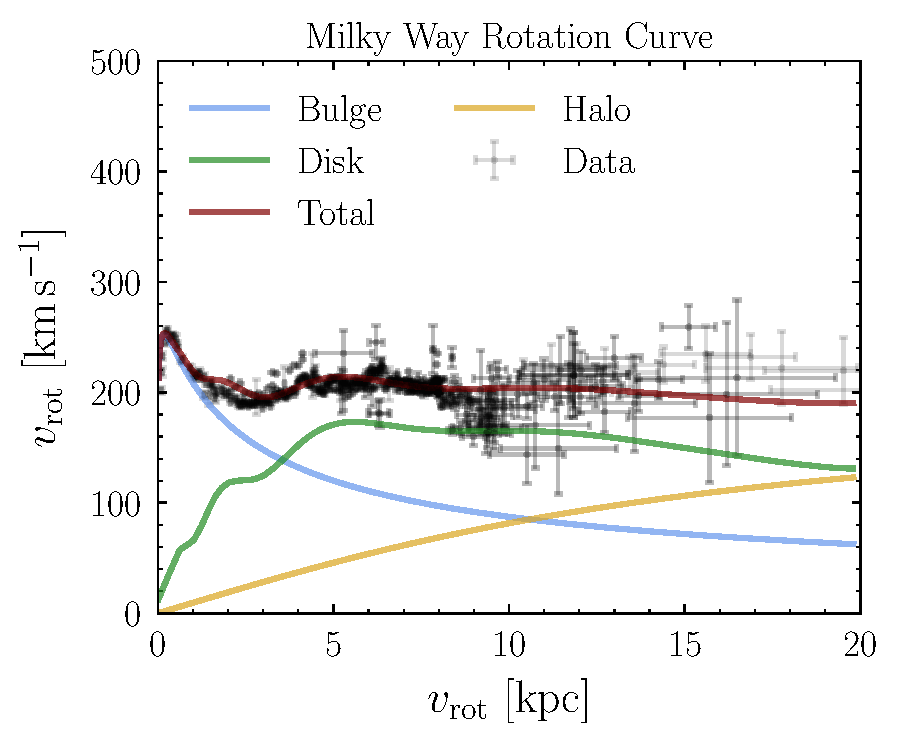
\includegraphics[width=0.5185\textwidth]{rotcurves.pdf}
 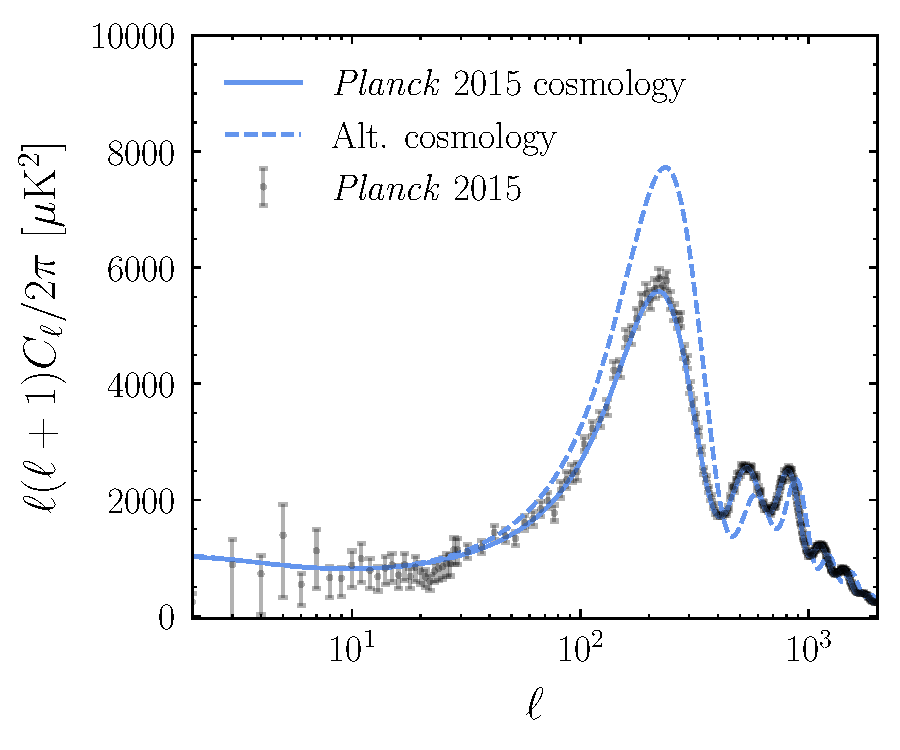
\includegraphics[width=0.528\textwidth]{cells.pdf}  
\caption{Caption}  
\label{fig:evidence}
\end{figure}


\section{(Particle) Nature of Dark Matter}
\label{sec:particledm}

Although the existence of dark matter is incontrovertible, its nature largely remains a mystery. These days, it is often implicitly assumed that when people are talking about detecting dark matter, say at a Xenon direct detection experiment or in gamma ray data, that this refers to a dark matter \emph{particle}. As touched upon above, this was by no means always the case -- early usage and references to dark matter usually referred to the existence of generic dark objects that would be too faint to be observed, such as dim stars or internebular material. The transition in usage from an adjective to a noun was a result of sociological changes within the particle physics and astrophysics communities, bringing the two closer after the missing mass problem had been firmly accepted in the 1970s. All the evidence amassed since then is consistent with dark matter being made up of a fundamental particle, or perhaps even the existence of an entire dark sector consisting of many particles with a rich set of properties and interactions.

Within the Standard Model, neutrinos---by virtue of being stable (or very long-lived), electrically neutral particles and not interacting strongly---contain some of the essential attributes for a particle dark matter candidate, and were discussed in this context early on. Cosmological effects of neutrinos were discussed throughout the 1960s and 1970s, pioneered by the work of Zeldovich and others, and their implications for the missing mass observed on (super-)galactic scales was discussed by Weinberg and others in the the late 1970s. Early simulations during the 1980s eventually showed that hot (relativistic) and cold (non-relativistic) particle dark matter would lead to very different outcomes for structure formation, leading to formation and collapse of larger structures---``top-down''---in the former case and a hierarchical ``bottom-up'' structure formation in the latter. Neutrinos, by virtue of being very light thermal relics, would be extremely relativistic during structure formation, and combined with these simulations early surveys of the local Universe were able to quickly disfavor their role as dark matter candidates. Nevertheless, along the way neutrinos served as a gateway particle in understanding the implications of new particles to observations on galactic, cluster and cosmological scales.

With no reason to be confined to the Standard Model, supersymmetry (SUSY) posits that nature may contain a spacetime symmetry relation bosons and fermions, requiring that for ever boson a fermion with the same quantum numbers must exist (and vice versa). This leads to the prediction of several new electrically neutral particles uncharged under the strong force. If some of these were stable, they could have played an important role in the history of our Universe and could conceivably make up some portion of dark matter. Supersymmetry took its modern form with a paper by Dimopolous and Georgi, who introduced the MSSM. In the MSSM, superpartners of the $Z$ boson, photon and two Higgses mix to form four particles, today known as neutralinos. R-parity conservation would prevent the lightest neutralino from decaying quickly after being created. Neutrinos have arguably been the most-discussed dark matter candidate. This is in part because supersymmetry, with its ability to enable gauge coupling unification and solve the electroweak hierarchy problem, is motivated in its own right, and the existence of a viable dark matter candidate is often seen as a desirable bonus.

Besides SUSY-motivated neutralinos, there is no shortage of viable particle DM candidates today, including but not limited to axions, sterile neutrinos and dark photons. The most general statements we can make regarding, for example, the mass of the dark matter particle are relatively unconstrained. $m_\text{scalar} \gtrsim 10^{-22}$\,eV for bosons, and $m_\text{fermion} \gtrsim 0.7$\,keV for fermions come from observations of DM halos around dwarf galaxies, and the requirement for particles to occupy a minimum phase-space volume according to the uncertainty principle and the Pauli exclusion principle respectively.

\subsection{Thermal Dark Matter}

There are several general and striking features pertaining to dark matter particles in thermal equilibrium with the Standard Model in the early Universe. In order for such a particle to freeze out of equilibrium and become a cold relic, it must be heavier that $\sim$keV mass. Additionally, in order to match the observed DM density, the DM particles must self-annihilate with a cross-section of $\sigma v\sim 10^{-26}$\,cm$^3$\,s$^{-1}$, which is strikingly close to the cross-section arising from the weak interaction. This fact holds for a large variety of electroweak-scale DM candidates, and given the theoretical arguments for the existence of new physics at electroweak scales, WIMPs have become the dominant particle dark matter paradigm and have motivated an extensive search program.

Searches for WIMPs are generally organized into three categories depending on the experimental detection strategy. Direct detection, which looks for the energy deposited when dark matter particles recoil against nuclei through the process $\text{SM}\,\chi\rightarrow\text{SM}\,\chi$, where $\chi$ is a DM particle. While the flux of WIMPs through a terrestrial detector can be large, the expected deposited energies and interact rates are very small, requiring large amounts of target material and exquisite control over backgrounds. Direct detection experiments have been able to set very strong limits on WIMP scenarios and have been able to exclude several baseline models, such as $Z$-mediated DM interactions--see~\cite{} for a recent review. The second class of searches involves the production of WIMPs at particle colliders like the Large Hadron Collider (LHC) through the process $\mathrm{SM}\,\mathrm{SM}\rightarrow\chi\,\chi$, usually in association with additionally visible particles emitted by initial or intermediate SM particles that can used to detect the event along with the missing energy characterizing the WIMP. 

The final strategy and the focus of this is indirect detection, which looks for the annihilation of DM particles into SM particles through the process $\chi\,\chi\rightarrow\mathrm{SM}\,\mathrm{SM}$. The nature of the SM particles depends on the specific DM model. The basic idea behind indirect detection is that annihilation processes will be taking place at higher rates in regions of the Universe that are dark matter rich, leading to an excess in production of SM particles which would then cascade on to photons, electrons, positrons and (anti)protons, some of which would eventually be detected with telescopes. In the next section, I will introduce some of the challenges associated with indirect detection searches and tools required to perform them. 

\section{Indirect Detection of Annihilating Dark Matter}
\label{sec:astrodm}

As noted above, for generic thermal WIMP scenarios where the DM can self-annihilate, its late-time abundance is set by the coupling of the DM particle to the Standard Model. The expected self-annihilation cross-section in this case is entirely predictive and we would expect an electroweak-scale cross-section around $\sigma v\sim 10^{-26}$\,cm$^3$\,s$^{-1}$, and DM particle mass of $\mathcal O($GeV-TeV). DM particles in this mass range annihilating to SM particles would produce secondary photons which would fall dominantly in the gamma-ray range. This regime is well-probed by today's gamma-ray telescopes, including the \emph{Fermi} Large Area Telescope, as well as several current and upcoming observatories. In this section, I will describe the ingredients necessary to calculate the expected DM annihilation flux and discuss common astrophysical search targets. 

\subsection{Tools for Indirect Detection}

A primary challenge for indirect detection is to estimate the annihilation flux that would be observed from a given astrophysical target or population. If the DM density at angular coordinates $\psi$ (describing the angle away from the Galactic plane) located at a line-of-sight distance $l$ from us is $n[r(l,\psi)]$, the annihilation rate per particle is given by
\begin{equation}
n[r(l,\psi)]\langle\sigma v\rangle = \frac{\rho[r(l,\psi)]}{m_\chi}\langle\sigma v\rangle.
\end{equation}
The total annihilation rate in a volume element $dV = l^2\,dl\,d\Omega$ is given by convolving this by the number of particles in the volume:
\begin{equation}
\frac{\rho[r(l,\psi)]}{m_\chi}\langle\sigma v\rangle \frac{\rho[r(l,\psi)]}{2m_\chi}dV.
\end{equation}
where the factor of 2 comes from avoiding double counting since two particles are involved in the annihilation. The total observed annihilation flux is given by:
\begin{equation}
\frac{d\Phi}{dE}(E,\Psi) = \frac{1}{4\pi}\int\,d\Omega\,dl\,\rho[r(l,\psi)]^2\frac{\langle\sigma v\rangle}{2m_\chi^2}\frac{dN}{dE}
\end{equation}
where $\frac{dN}{dE}$ gives the number of photons produced per annihilation, for a given annihilation channel. The annihilation cross-section can often be factorized out of the integral, but this is not possible if the cross section has a strong velocity-dependence, e.g. in $p$-wave annihilation scenarios (see for more details). All astrophysical information is contained in the so-called J-factor, which is the line-of-sight integral along a given direction of the squared dark matter density. In the simplest scenarios where this is possible, the annihilation flux factorizes as
\begin{equation}
\frac{d\Phi}{dE}(E,\Psi) = \frac{\langle\sigma v\rangle}{8\pi m_\chi^2}\frac{dN}{dE}\int\,d\Omega\,dl\,\rho[r(l,\psi)]^2
\end{equation}
where $J\equiv\int\,d\Omega\,dl\,\rho[r(l,\psi)]^2$ encapsulate the astrophysical dependence of the flux, and objects with higher $J$-factors typically make more interesting targets for indirect detection searches. However, a high $J$-factor by itself does not guarantee a good annihilation target. This must additionally be balanced with how well the systematic uncertainties on both the properties of the source population as well as astrophysical backgrounds can be controlled, and the ability to leverage the statistics of the underlying DM signal.

\subsection{Sources of Gamma Rays from Annihilating Dark Matter}

An important challenge in indirect detection is accurately characterizing the DM signal and associated statistics. This often involves astrophysical input as well as input from observations at other wavelengths and $N$-body simulations in order to predict the annihilation flux and accurately characterize the associated uncertainties. Roughly, the $J$-factor scales as $\sim(\int\rho^2\,dV)/d^2$, where $\rho$ is the DM density distribution and $d$ the distance of the object from us. The following objects are generally considered as targets in DM annihilation searches: 
\begin{itemize}
\item \emph{Dwarf galaxies}: Dwarf spheroidal satellite galaxies (dSphs) of the Milky Way have traditionally been considered excellent targets for DM annihilation searches. They are dark matter dominated and have high mass-to-light ratios, making them relatively clean targets for annihilation searches. There have been about 45 dSphs discovered recently by surveys like SDSS and DES, and combined searches have been able to place some of the strongest constraints on annihilation scenarios. The relevant $J$-factors are from well-characterized, however -- assumptions about, \emph{e.g.}, the dSph halo profile and membership criteria for stars used to infer the halo properties can lead to large uncertainties.
\item \emph{Milky way halo}: Our own Galaxy is the brightest source of DM emission in the sky. Searches in the inner Galaxy, where the signal is expected to be the brightest, have yielded an excess emission whose spatial and spectral properties can be consistent with those of a DM annihilation signal (\emph{e.g.}, a $\sim$40\,GeV WIMP annihilation to $b\bar b$ with approximately thermal cross section), often called the Galactic Center Excess. This region of the sky is complicated by the presence of substantial and difficult Galactic foregrounds which are difficult to characterize, which complicates the interpretation of any signal and/or limit from this region. Indeed, recent results based on studying the statistics of photons in the region show that excess is more consistent with emission from an unresolved population of point sources, rather than a dark matter signal.

Another class of searches focuses on looking for DM emission from the Milky Way at higher Galactic latitudes, where the signal is still appreciable but Galactic foregrounds are much lower. These studies necessitate being able to accurately characterize the Galactic foreground emission over larger regions of the sky, and a careful consideration of this effect yields strong limits on thermal WIMPs.

\item \emph{Galactic substructure}: Hierarchical bottom-up structure formation necessitates the existence of substructure within galaxies. These would be dark objects with little or no stellar activity, in contrast to classical and ultrafaint dwarfs mentioned above, which makes it impossible to localize them and look for their gamma ray emission. Traditional searches rely on characterizing the emission from unassociated gamma ray sources as seen by \emph{Fermi} as potentially coming from annihilation DM in individual subhalos, and comparing observations to expectations based on $N$-body simulations.

An orthogonal and promising approach is to study and look for the signature associated with DM annihilation from a population of sub-threshold subhalos using the methods described in Chapters 2 and 3 of this thesis. 

\item \emph{Extragalactic galaxies and clusters}: Searches for DM annihilation in extragalactic targets have traditionally been complicated by the difficulty in characterizing the DM properties of extragalactic halos (and consequently, the DM annihilation signal) and the presence of potentially significant astrophysical emission. Studies of emission from individual, nearby clusters, the integrated, isotropic emission from background halos, and cross-correlation of gamma rays with local catalogs of galaxies and large-scale structure. These studies typically (for realistic assumptions) do not attain sensitivity to thermal WIMP scenarios. Chapters 4 and 5 of this thesis focus on developing methods to systematically characterize the dark matter emission from extragalactic clusters, along with the associated uncertainties, and looking for this structure in gamma ray data. 
\end{itemize}

Future TeV-scale observatories

\section{Summary}
\label{sec:summary}


% \begin{itemize}
% \item History of dark matter

% \item Particle dark matter
% \item The case for WIMPs 
% \item Dark matter searches
% \end{itemize}